\documentclass[11pt]{article}
\usepackage[utf8]{inputenc}
\usepackage{listings}
\usepackage{xcolor}
\usepackage{graphicx}
\usepackage{hyperref}

% set the page margin
\usepackage[margin=1in]{geometry}

\definecolor{codegreen}{rgb}{0,0.6,0}
\definecolor{codegray}{rgb}{0.5,0.5,0.5}
\definecolor{codepurple}{rgb}{0.58,0,0.82}

\lstdefinestyle{codestyle}{
    commentstyle=\color{codegreen},
    keywordstyle=\color{blue},
    stringstyle=\color{codepurple},
    basicstyle=\ttfamily\small,
    breakatwhitespace=false,
    breaklines=true,
    keepspaces=true,
    showspaces=false,
    showstringspaces=false,
    numbers=left,
    numberstyle=\tiny\color{codegray},
    stepnumber=1,
    tabsize=4
}

\lstset{style=codestyle}

\title{Report: B+ Tree Implementation in Python}
\author{Chaoren Wang, 122090513}
\date{\today}

\begin{document}

\maketitle

\section{Introduction}
This report details the implementation of a B+ Tree data structure in Python. The implementation includes all core functionalities required for a B+ Tree:
\begin{itemize}
    \item Insertion with node splitting and redistribution
    \item Deletion with node merging and rotation (i.e. borrowing from siblings)
    \item Search operations using binary search
    \item Optional display functionality for ASCII tree visualization
\end{itemize}

The implementation maintains the essential properties of B+ Trees, including balanced height, ordered keys, and linked leaf nodes for efficient range queries. 

The code is designed to be both efficient and maintainable, with a focus on clear separation of concerns and proper documentation. Besides, logging and debugging features are also implemented for development and testing purposes. Four testcases mentioned in Lecture 8 are provided to test the correctness of the implementation.

\section{Design \& Implementation}

\subsection{Core Classes}
The implementation consists of two main classes:
\begin{itemize}
    \item \texttt{BPlusTreeNode}: Represents individual nodes in the tree, including leaf nodes and non-leaf nodes
    \item \texttt{BPlusTree}: Manages the tree structure and operations, providing APIs for insertion, deletion, search, and display
\end{itemize}

\subsection{Key Design Choices}

\paragraph{Node Structure} Every node (including leaf nodes and non-leaf nodes) maintains lists for keys and values separately; Leaf nodes are doubly-linked for efficient range queries; Parent references are maintained for bottom-up operations (like merging and rotation).

\paragraph{Operation Implementation} For four operations (insertion, deletion, search, and display), the implementation follows the lecture notes closely: (1) Insertion uses recursive splitting with bottom-up propagation; (2) Deletion implements both rotation and merging strategies; (3) Search utilizes binary search within nodes; (4) Optional \texttt{--plain} argument provides a plain display mode without ASCII tree format.

\paragraph{OOP Design} The implementation is designed using object-oriented programming (OOP) techniques, which helps to keep clean code and easy to understand.

\subsection{Challenges and Solutions}

\subsubsection{Challenge 1: Node Splitting}
The main challenge was maintaining tree properties during node splits after insertion. 

When inserting a new key, the node needs to be split if it is full. This involves redistributing keys and updating parent references. However, redistribution is not a trivial task, specifically when it involves updating the parent's keys. 

To solve this, I implemented \texttt{node.split} and \texttt{tree.\_merge\_into\_parent} functions to handle the splitting and merging process, which is called recursively when necessary.

\subsubsection{Challenge 2: Deletion Redistribution}

When deleting a key, the node needs to be redistributed if it has insufficient keys. This involves borrowing keys from siblings or merging with siblings and updating the parent keys.

More challenging, when parents' keys are updated, the redistribution process needs to be recursively applied to the parent nodes until the tree meets the requirement.

To solve this, I implemented \texttt{node.remove} and \texttt{tree.\_update\_parents} functions to handle the redistribution process. After deletion, the code will first try to borrow keys from siblings by calling \texttt{tree.\_left\_rotate} and \texttt{tree.\_right\_rotate}; if rotation is not possible, it will merge with siblings by \texttt{tree.\_left\_redistribute} and \texttt{tree.\_right\_redistribute}, and then update the parent keys by \texttt{tree.\_update\_parents}.


\section{Code Usage}

The code is implemented in \texttt{bptree.py}, which is purely written in Python 3.12.7 without any external dependencies.

\subsection{Basic Operations}
Here's how to use the basic operations:

\begin{lstlisting}[language=Python]
# Create a B+ Tree with order 4
tree = BPlusTree(4)

# Insert values
tree.insert(10)
tree.insert(20)
tree.insert(5)

# Search for a value
tree.find(10)  # Outputs: ">> Key found: 10"

# Delete a value
tree.delete(20)

# Display the tree
tree.display()
\end{lstlisting}

\subsection{Example Output}
Some example outputs are shown in Figure \ref{fig:basic}, \ref{fig:insertion}, \ref{fig:deletion}, \ref{fig:parent_merge}, and \ref{fig:deletion_with_merge}. These outputs are produced by running with \texttt{--debug} option. For plain display mode running with \texttt{--plain} option, see Figure \ref{fig:plain}.

\begin{figure}[h!]
    \begin{minipage}[t]{0.48\textwidth}
        \centering
        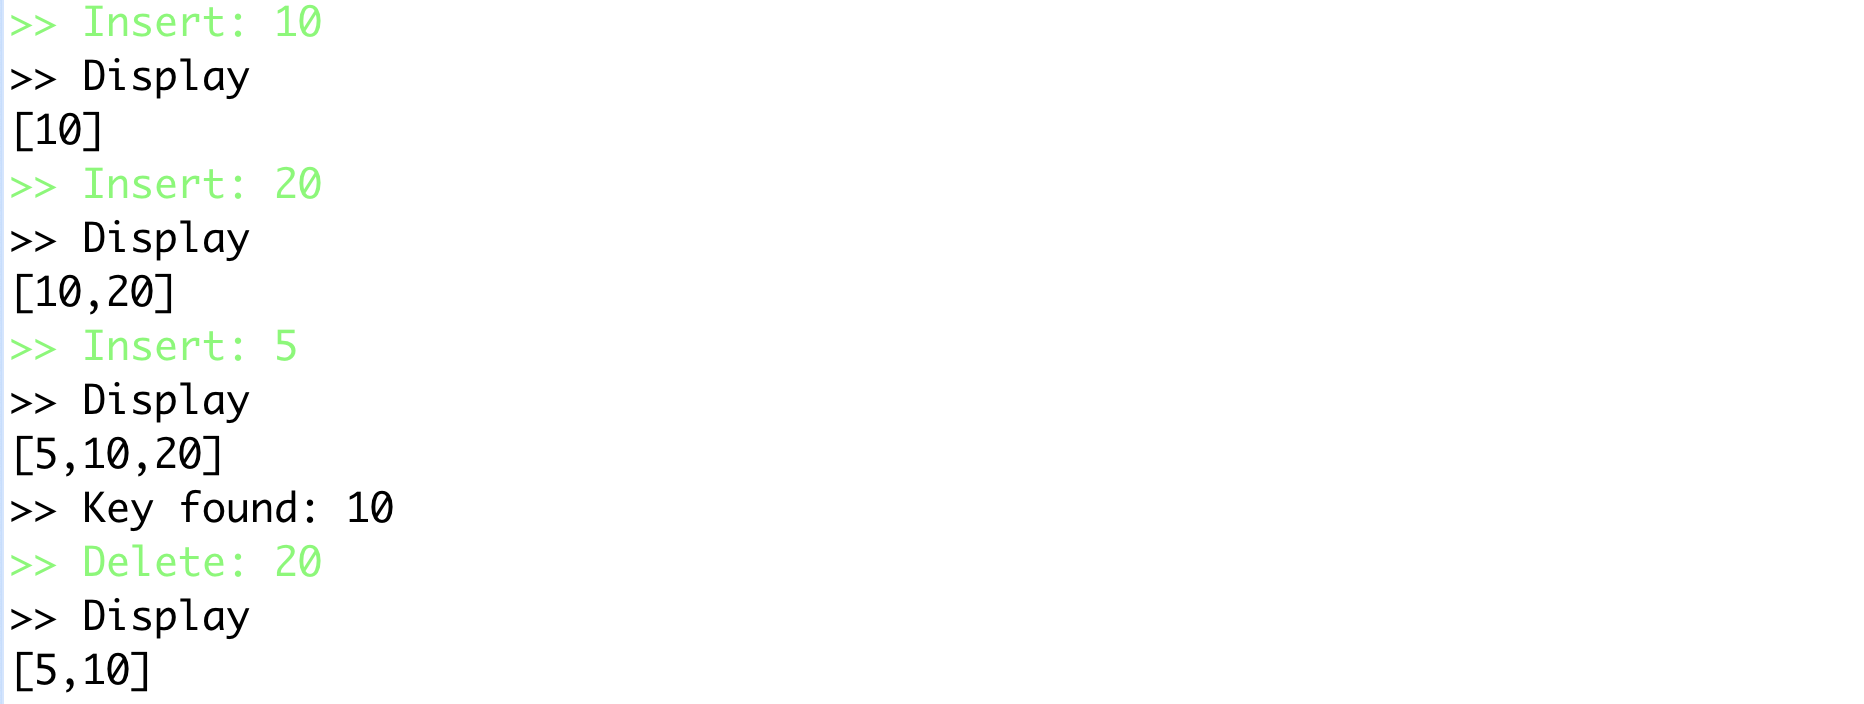
\includegraphics[width=\textwidth]{figs/basic.png}
        \caption{Basic operations}
        \label{fig:basic}
    \end{minipage}
    \hfill
    \begin{minipage}[t]{0.48\textwidth}
        \centering
        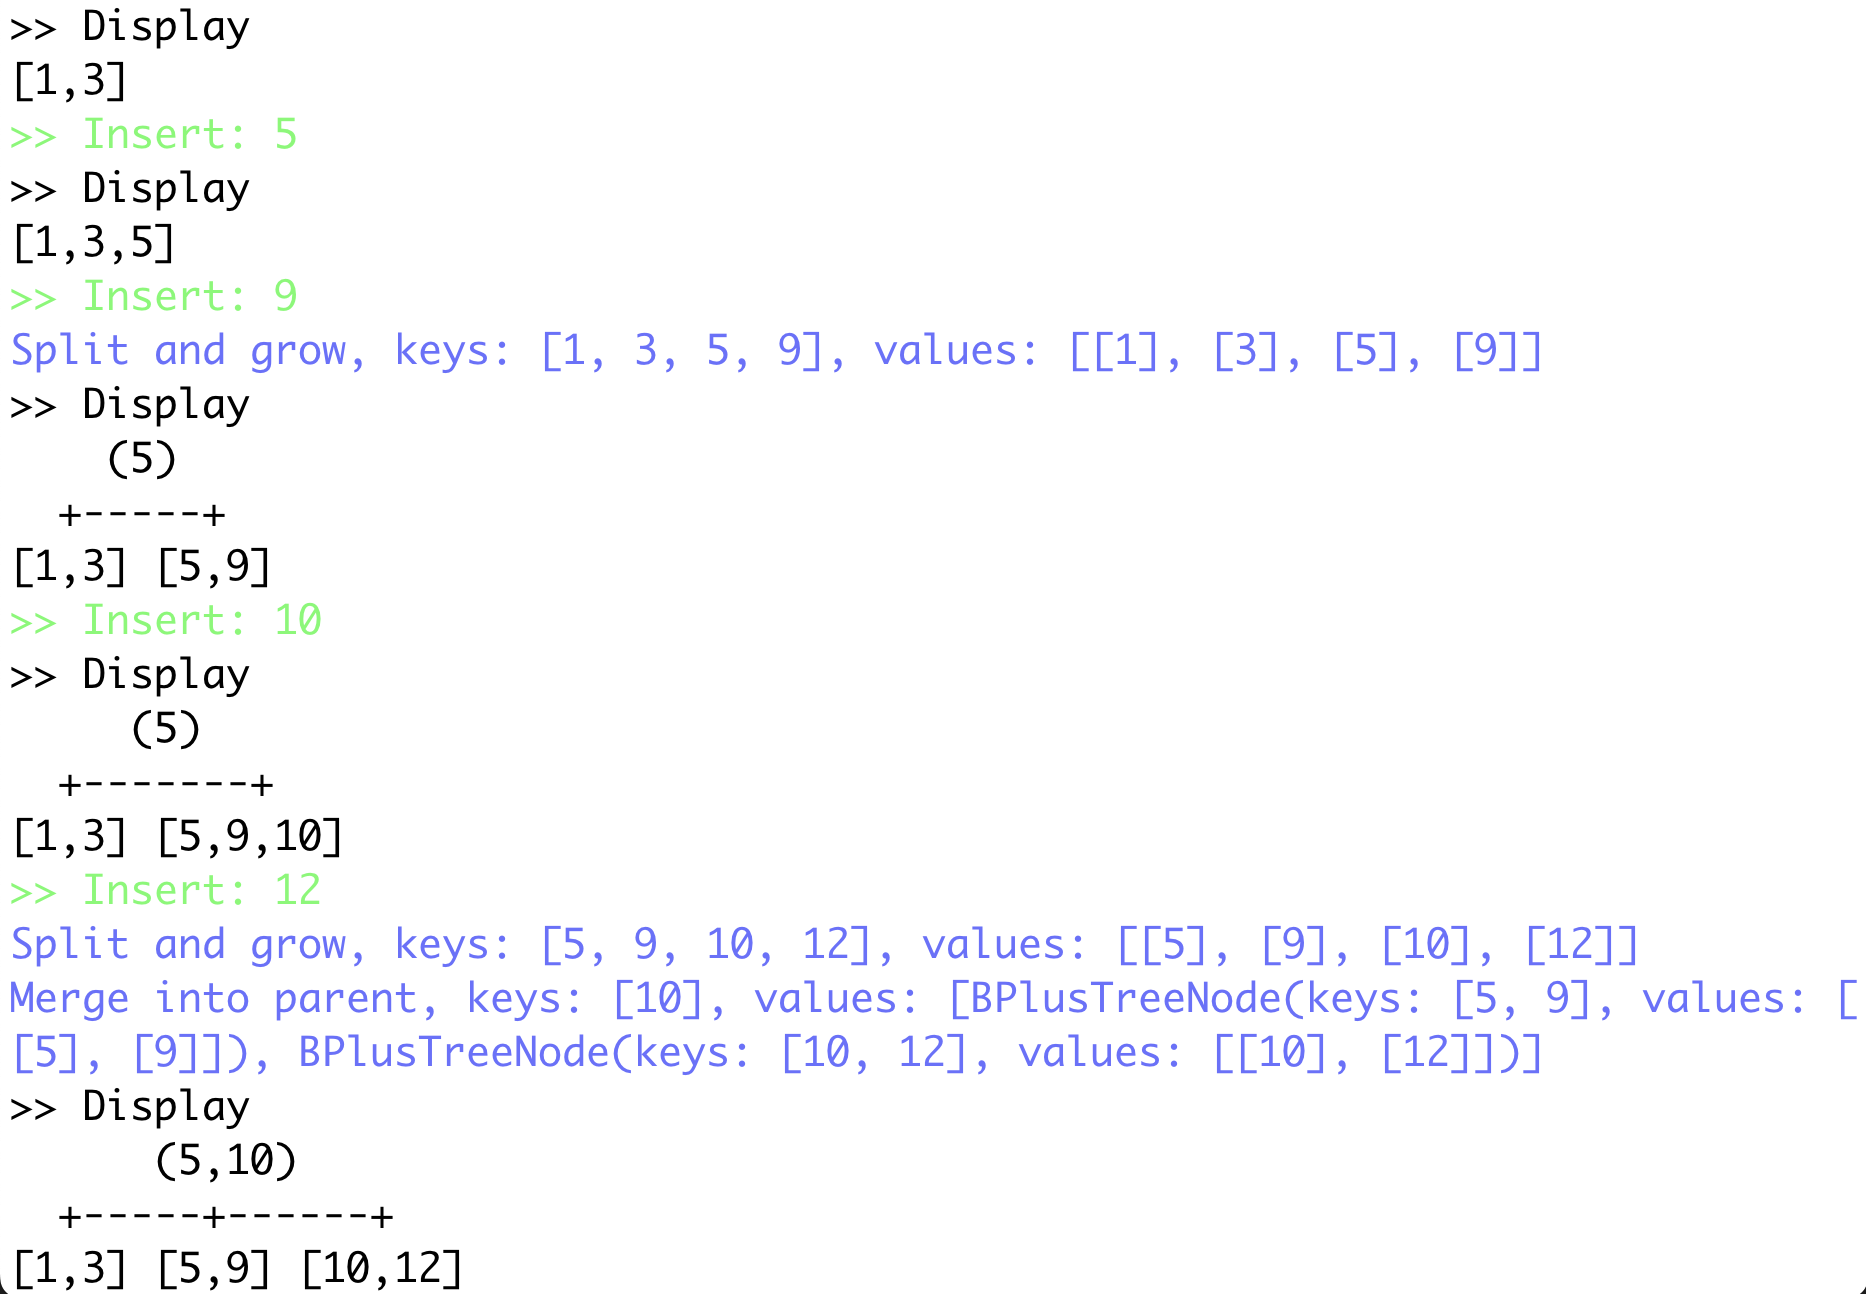
\includegraphics[width=\textwidth]{figs/insertion.png}
        \caption{Insertion operation with split and grow}
        \label{fig:insertion}
    \end{minipage}
\end{figure}

\begin{figure}[h!]
    \begin{minipage}[t]{0.48\textwidth}
        \centering
        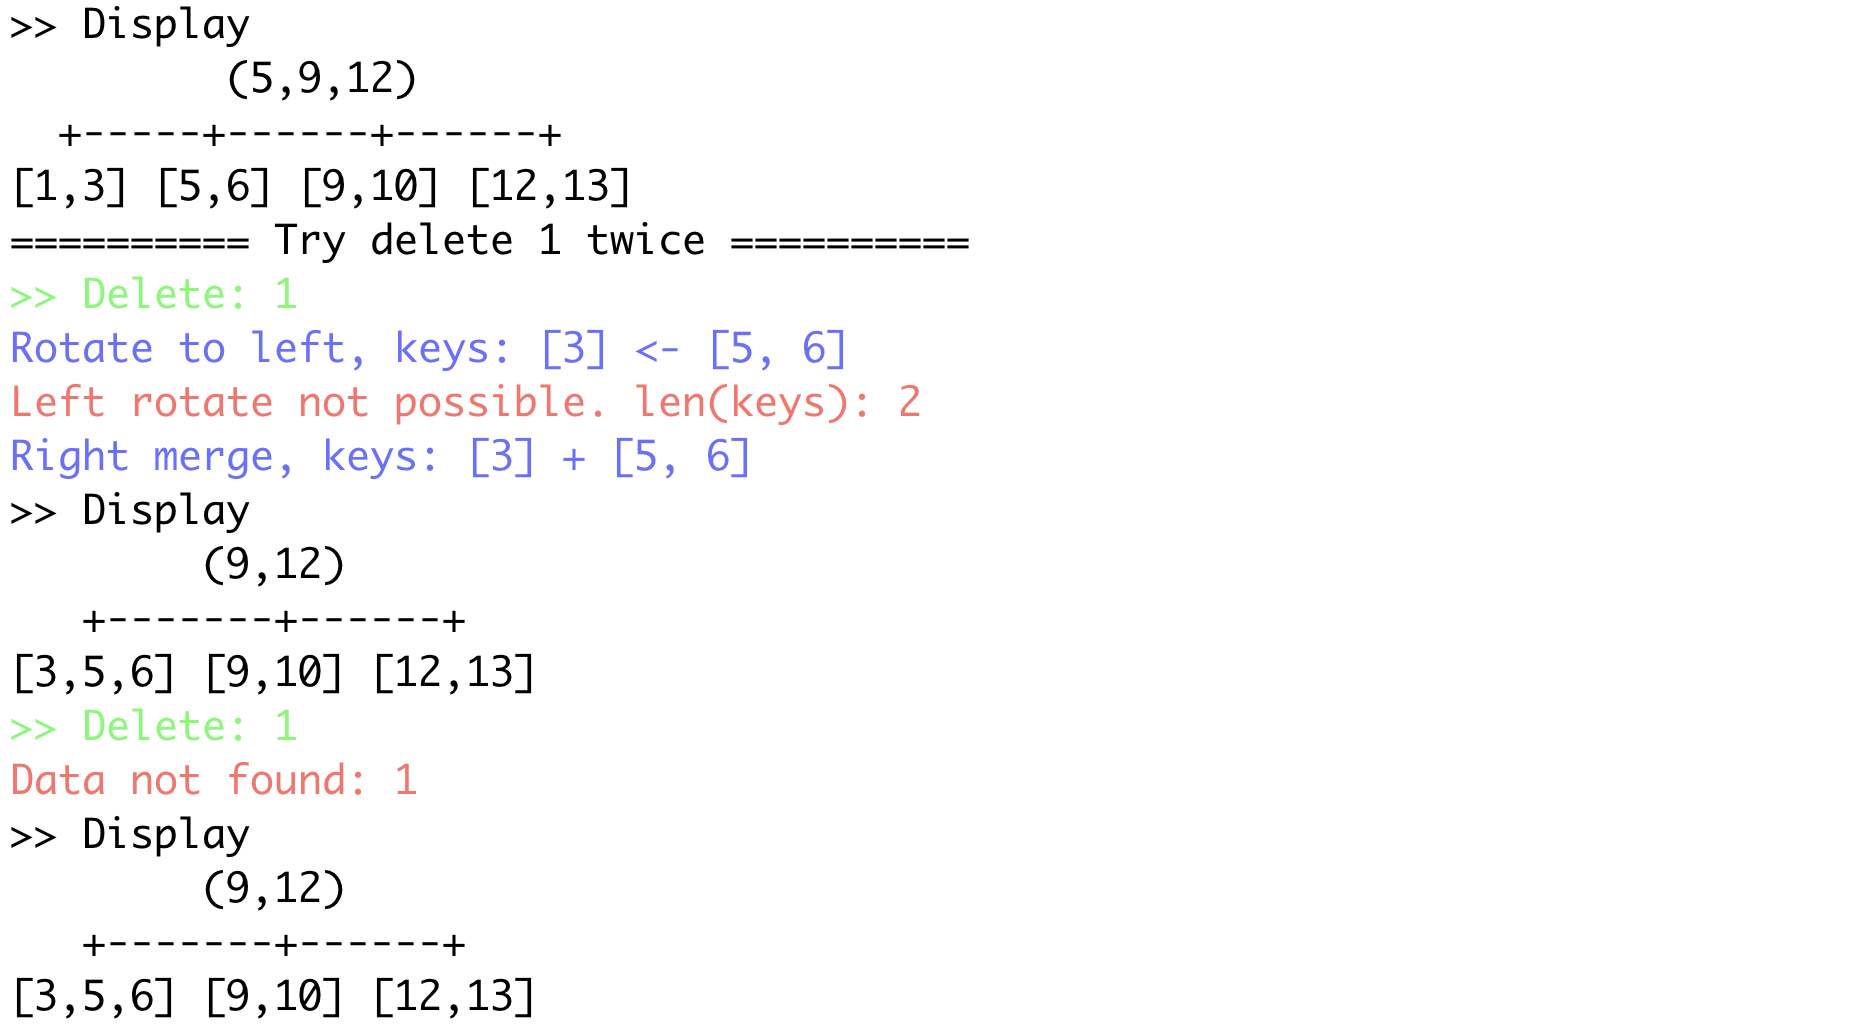
\includegraphics[width=\textwidth]{figs/deletion.png}
        \caption{Deletion operation with rotation}
        \label{fig:deletion}
    \end{minipage}
    \hfill
    \begin{minipage}[t]{0.48\textwidth}
        \centering
        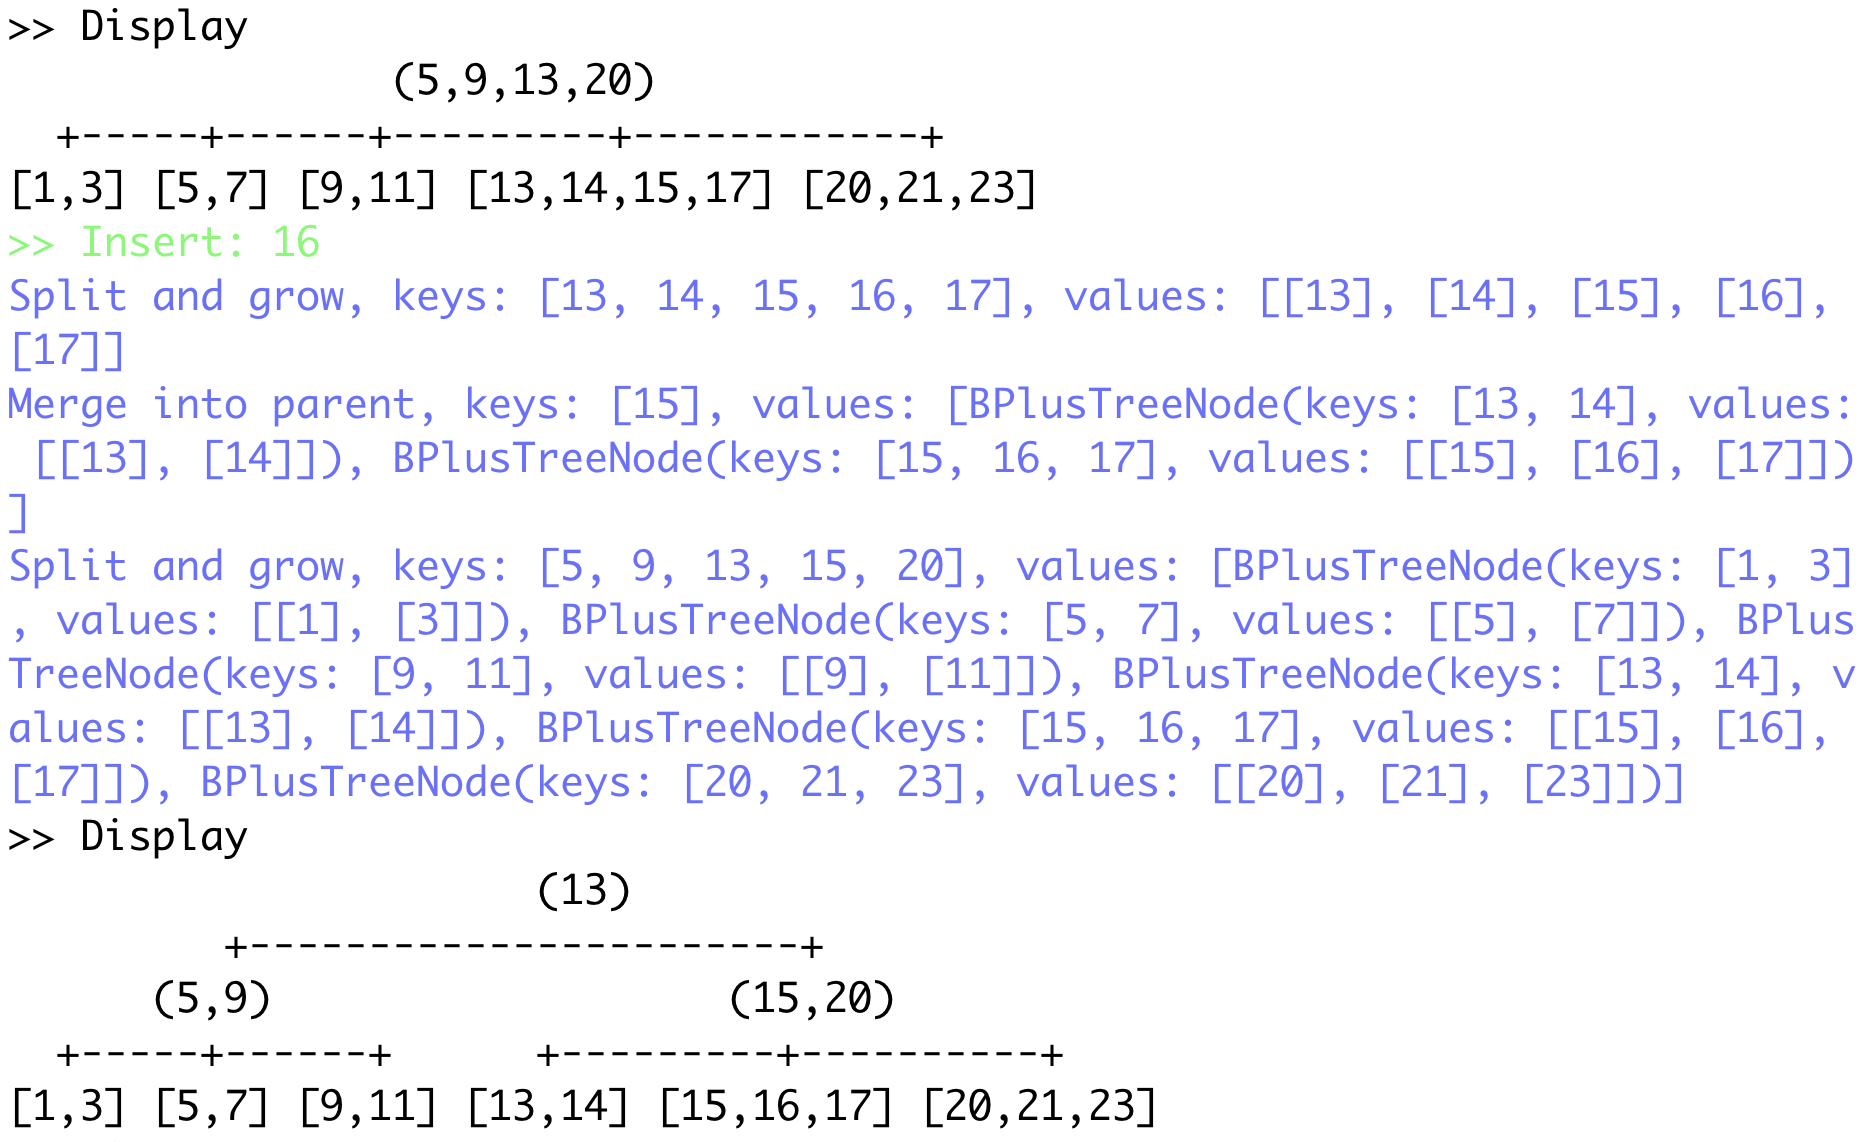
\includegraphics[width=\textwidth]{figs/parent_merge.png}
        \caption{Insertion operation with merge into parent}
        \label{fig:parent_merge}
    \end{minipage}
\end{figure}

\begin{figure}[h!]
    \begin{minipage}[t]{0.48\textwidth}
        \centering
        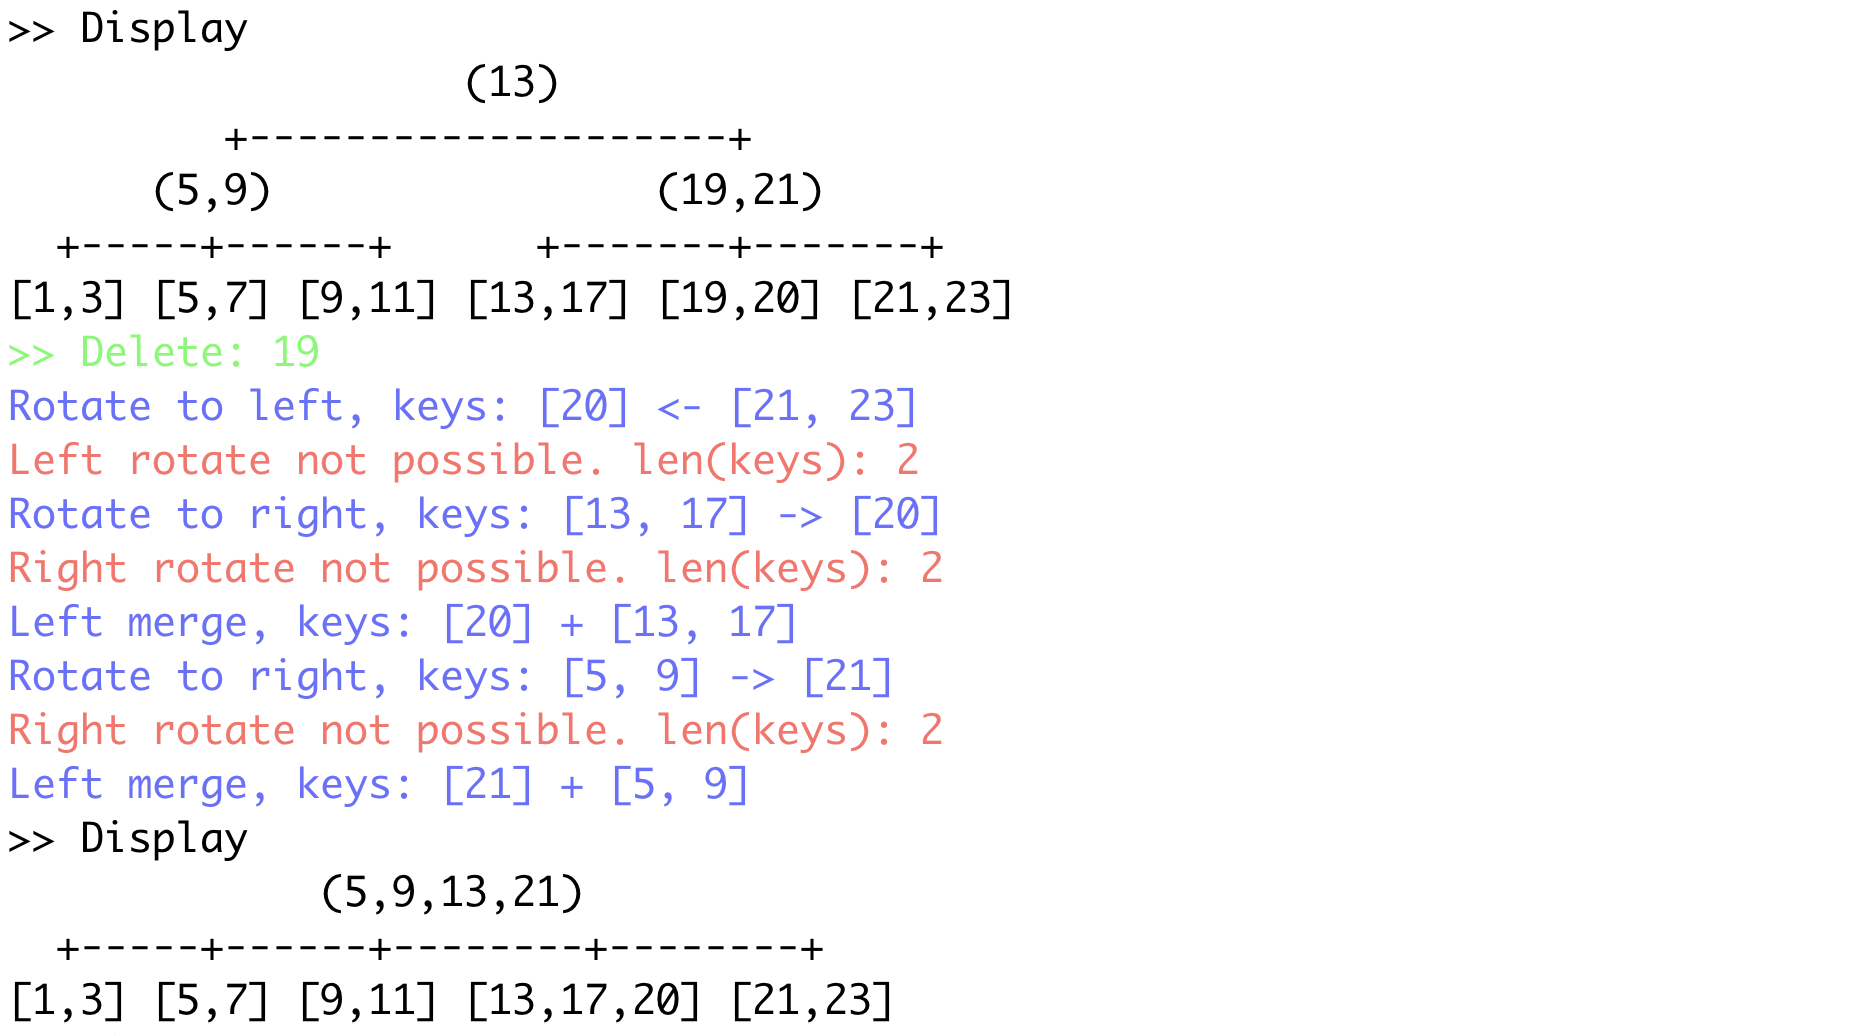
\includegraphics[width=\textwidth]{figs/deletion_with_merge.png}
        \caption{Deletion operation with merge}
        \label{fig:deletion_with_merge}
        \end{minipage}
    \hfill
    \begin{minipage}[t]{0.48\textwidth}
        \centering
        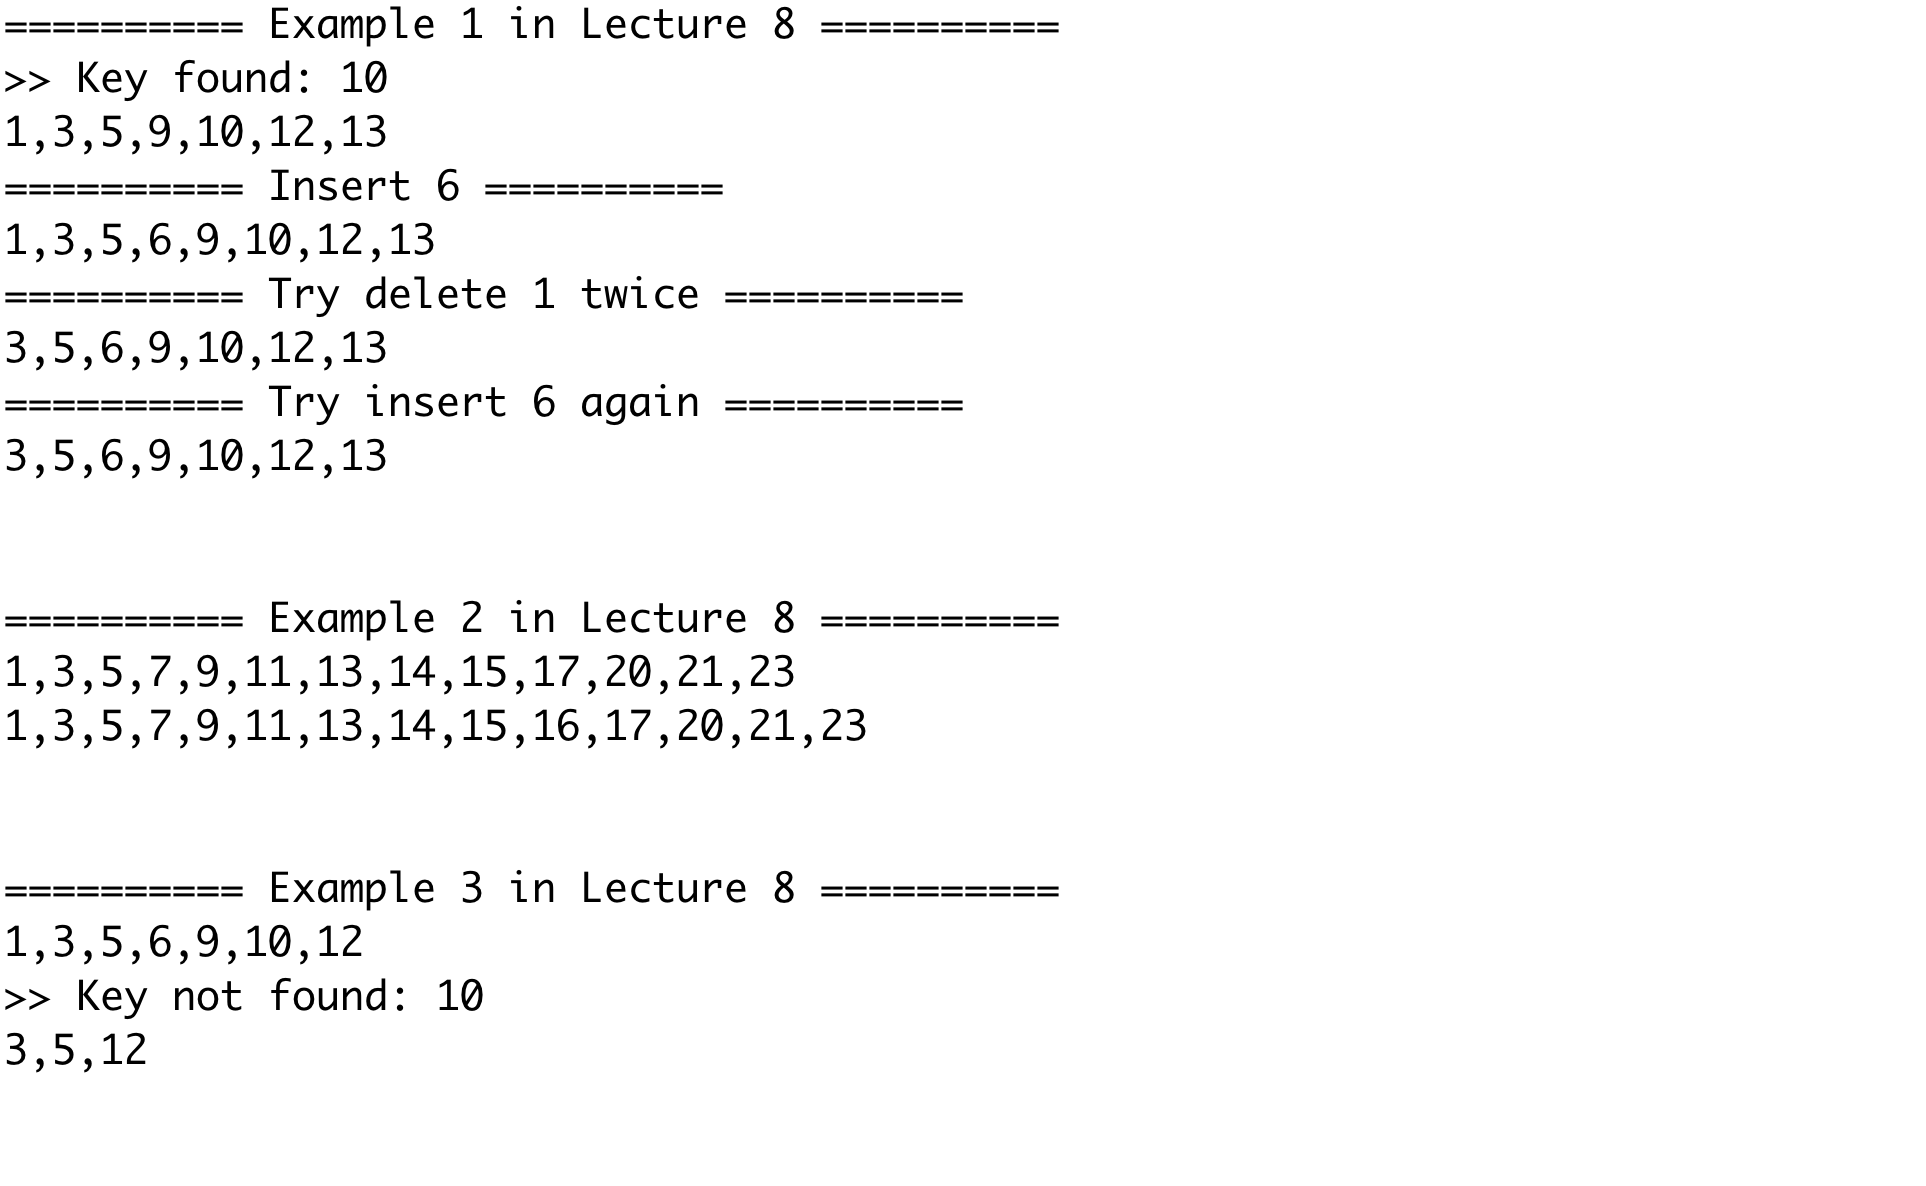
\includegraphics[width=\textwidth]{figs/plain.png}
        \caption{Plain display mode}
        \label{fig:plain}
    \end{minipage}
\end{figure}


\subsection{Additional Features}
The implementation includes additional features: (1) Debug logging for operation tracking; (2) Command-line arguments for display options; (3) Colored output for better visualization.

\subsection{Running the Code}
The code can be run with various options:
\begin{lstlisting}[language=bash]
python bptree.py            # Only show tree when calling display()
python bptree.py --display  # Show tree after each operation
python bptree.py --logging  # Enable colored operation logging
python bptree.py --debug    # Enable --display and --logging
python bptree.py --plain    # Show results without ASCII format: this format aligns the assignment requirement, compatible with other options
\end{lstlisting}

\section{Conclusion}
The implemented B+ Tree maintains O(log n) complexity for all operations while preserving the core properties of B+ Trees. By designing and developing the code, I have a deeper understanding of B+ Trees and their operations, also exercised my coding skills especially in involving recursively updating after a single operation.

\end{document}